\section{Quantum Multi-Party Computation}

\begin{refsection}

\subsection{Our Approach}
\subsubsection{Message Access}
Let's consider 2 parties, Alice and Bob. Alice has a set $M = \{m_0,m_1\}$ of messages and Bob has the index, $i$, of the message he wants to receive from Alice, $m_i$.\\
For this example we will be assuming that $i=1$ and $M = \{11,10\}$. Both messages are 2-bit binary numbers.
\begin{enumerate}
%%%%%%%%%%%%%%%%%%%%%%%%%%%%%%%%%%%%%%%%%%%%%%%%%%%%%%%%%%%%%%%%%%%%%%%%%%%%%%%%%%%%%%%%%%%%%%%%%%%%%%%%%%%%%%%%%%%%%%%%
\item Bob generates a 4-bit key, $K_b=0111$ where only the bits of indexes $2i$ and $2i+1$ are known ($C$) to him. Since i=1, Bob only knows the last 2 bits of $K_b$. The remaining 2 bits of $K_b$ are random ($R$), thus unknown to Bob.
\renewcommand{\figurename}{Figure}
\begin{figure}[H]
\centering
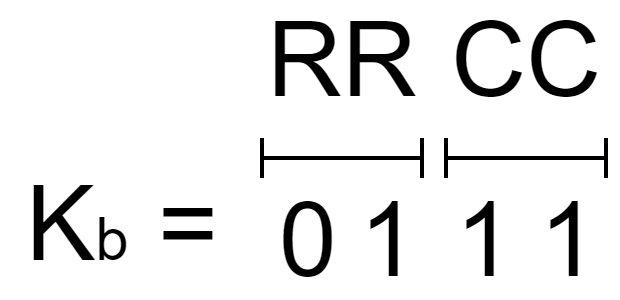
\includegraphics[width=.25\linewidth]{./figures/mpc/mpc_bob_key}
\caption{Known ($C$) and Unknown ($R$) bits from Bob's perspective }
\label{fig:knownbob}
\end{figure}
%%%%%%%%%%%%%%%%%%%%%%%%%%%%%%%%%%%%%%%%%%%%%%%%%%%%%%%%%%%%%%%%%%%%%%%%%%%%%%%%%%%%%%%%%%%%%%%%%%%%%%%%%%%%%%%%%%%%%%%%
\item Bob sends to Alice the set $I = \{2,3\}$ corresponding to the indexes of the bits known to him.
%%%%%%%%%%%%%%%%%%%%%%%%%%%%%%%%%%%%%%%%%%%%%%%%%%%%%%%%%%%%%%%%%%%%%%%%%%%%%%%%%%%%%%%%%%%%%%%%%%%%%%%%%%%%%%%%%%%%%%%%
\item Alice generates a 4-bit key, $K_a=1011$ where the last 2 bits of $K_a$ must be the same as the last 2 of $K_b$. All 4 bits from the key
are unknown to Alice. She doesn't know which 2 bits from $K_a$ are equal to $K_b$ (only Bob has that information),i.e., from her perspective
all bits are random.
\renewcommand{\figurename}{Figure}
\begin{figure}[H]
\centering
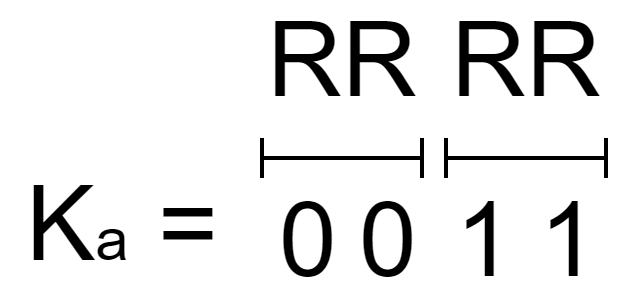
\includegraphics[width=.25\linewidth]{./figures/mpc/mpc_alice_key}
\caption{Known ($C$) and Unknown ($R$) bits from Alice's perspective }
\label{fig:knownalice}
\end{figure}
%%%%%%%%%%%%%%%%%%%%%%%%%%%%%%%%%%%%%%%%%%%%%%%%%%%%%%%%%%%%%%%%%%%%%%%%%%%%%%%%%%%%%%%%%%%%%%%%%%%%%%%%%%%%%%%%%%%%%%%%
\item Alice encrypts the messages with $K_a$ and sends the encrypted information to Bob. In this example, $1101$ will be sent to Bob.
\renewcommand{\figurename}{Figure}
\begin{figure}[H]
\centering
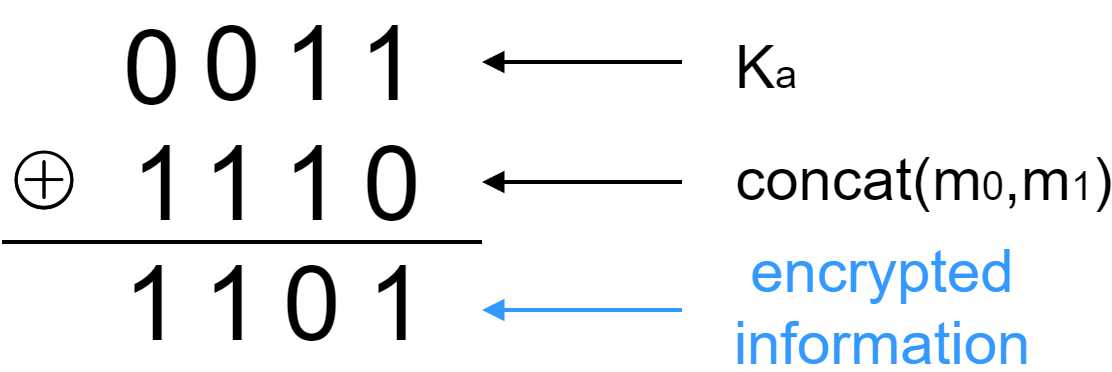
\includegraphics[width=.4\linewidth]{./figures/mpc/mpc_message_encrypting}
\caption{Alice encrypts the messages with $K_a$}
\label{fig:mpcencryption}
\end{figure}
%%%%%%%%%%%%%%%%%%%%%%%%%%%%%%%%%%%%%%%%%%%%%%%%%%%%%%%%%%%%%%%%%%%%%%%%%%%%%%%%%%%%%%%%%%%%%%%%%%%%%%%%%%%%%%%%%%%%%%%%
\item Bob decrypts the information received from Alice with $K_b$ and retrieves the message $m_1$, which correspond to bits of indexes 2 and 3 (since $i=1$).\\
The first two bits of the decrypted information do not represent $m_0$.
\renewcommand{\figurename}{Figure}
\begin{figure}[H]
\centering
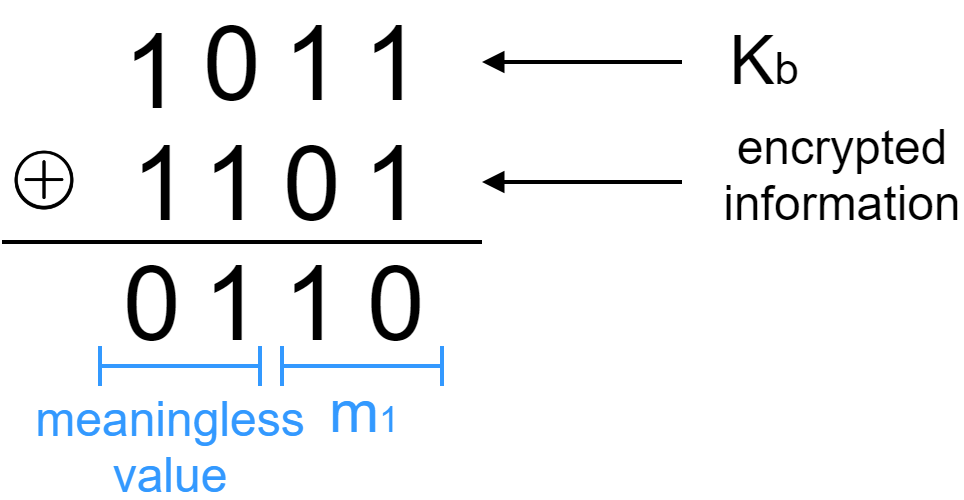
\includegraphics[width=.4\linewidth]{./figures/mpc/mpc_message_decrypting}
\caption{Bob decrypts the information with $K_b$}
\label{fig:mpcdecryption}
\end{figure}
\end{enumerate}

\subsubsection{The Millionaire' Problem}
%Complete this section
\subsubsection{Average Value}
%Complete this section



% bibliographic references for the section ----------------------------
\clearpage
\printbibliography[heading=subbibliography]
\end{refsection}
\addcontentsline{toc}{subsection}{Bibliography}
\cleardoublepage
% ---------------------------------------------------------------------